\chapter{Classic Algorithms}


\section{Greedy Algorithm}

\subsection{Clustering Problem}
Consider the following weighted graph. One can interpret the weights of the edges as the similarity between nodes. For instance, the nodes can correspond to different images in a dateset, and we draw an edge between two such images if they are comparable in some sense, where the weight of the edge is the similarity level between the images. The problem is given the weighted graph and an specified number of ``\emph{clusters}'' or ``\emph{categories}'', we want to group the nodes in a way that cost of the clustering is as small as possible. The \emph{cost} of clustering is the maximum weight of edges that are between two categories.
\begin{figure}[h!]
	\centering
	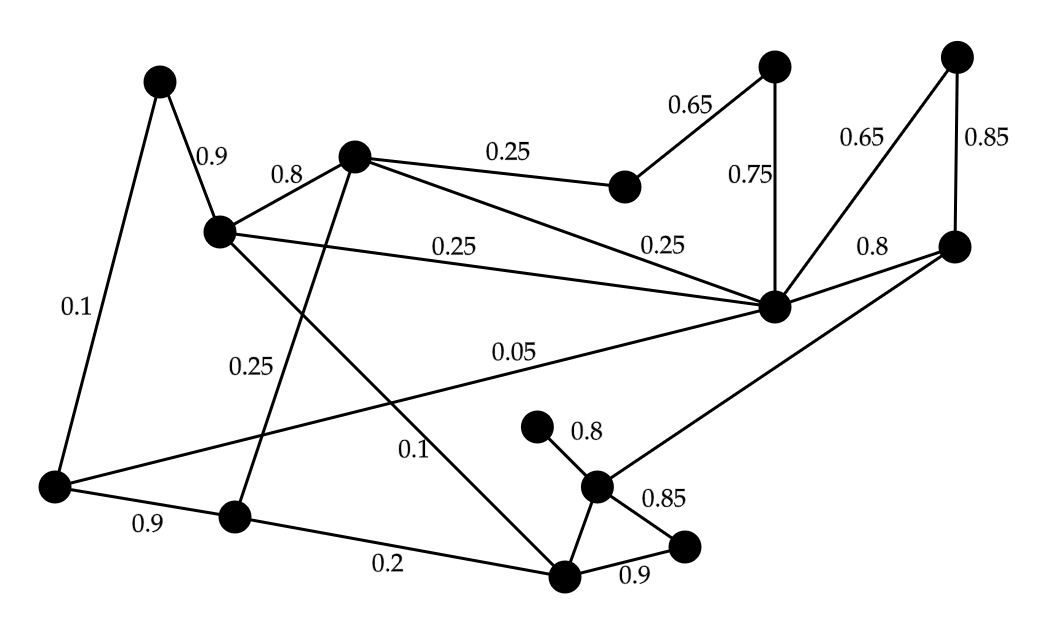
\includegraphics[width=0.7\linewidth]{Images/graphGreedyClustering}
	\label{fig:graphgreedyclustering}
\end{figure}
\FloatBarrier

Assume that the given weighted graph above, we want to categorize the nodes into 5 clusters. We follow the following greedy algorithm:

\begin{itemize}[align=left]
	\item[\emph{input}:] Given weighted graph $ G $ ($ n $ nodes, $ m $ edges) and number of clusters $ c $:
	\item[\emph{do:}] Sort the edges $ e_i $ in decreasing order of their weight.
	\item[\emph{do:}] make every node to be its own cluster.
	\item[\emph{define:}] $ C \leftarrow n $: number of current clusters
	\item[\emph{while:}] $ C \neq c $ iterate over $ E $
	\begin{itemize}
		\item[\emph{do:}] remove $ e_i $ from $ E $
		\item[\emph{if:}] adjacent nodes $ p_1,p_2 $ to $ e_i $ are not in the same category
		\begin{itemize}
			\item[\emph{do:}] join the categories of $ p_1 $ and $ p_2 $.
			\item[\emph{do:}] $ C \leftarrow C-1 $.
		\end{itemize}
	\end{itemize}
	
\end{itemize}


\begin{figure}[h!]
	\centering
	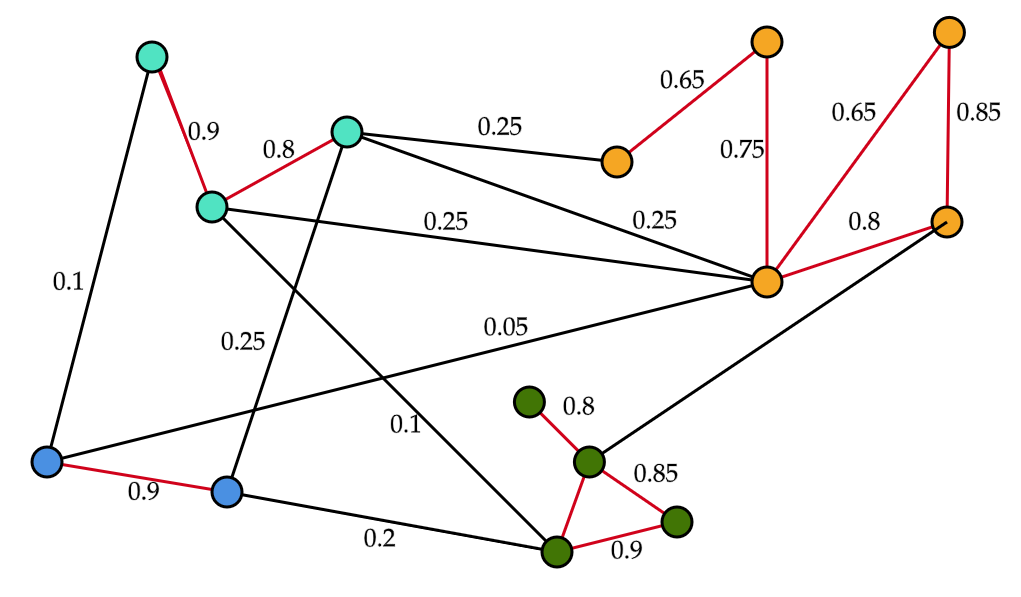
\includegraphics[width=0.7\linewidth]{Images/graphGreedyClustering_Clustered.png}
	\label{fig:graphgreedyclustering}
\end{figure}
